\documentclass[a4paper]{article} 
\addtolength{\hoffset}{-2.25cm}
\addtolength{\textwidth}{4.5cm}
\addtolength{\voffset}{-3.25cm}
\addtolength{\textheight}{5cm}
\setlength{\parskip}{0pt}
\setlength{\parindent}{0in}

\usepackage[square,sort,comma,numbers]{natbib}
\usepackage{blindtext} % Package to generate dummy text
\usepackage{charter} % Use the Charter font
\usepackage[utf8]{inputenc} % Use UTF-8 encoding
\usepackage{microtype} % Slightly tweak font spacing for aesthetics
\usepackage{amsthm, amsmath, amssymb} % Mathematical typesetting
\usepackage{float} % Improved interface for floating objects
\usepackage{hyperref} % For hyperlinks in the PDF
\usepackage{graphicx, multicol} % Enhanced support for graphics
\usepackage{xcolor} % Driver-independent color extensions
\usepackage{pseudocode} % Environment for specifying algorithms in a natural way
\usepackage[yyyymmdd]{datetime} % Uses YEAR-MONTH-DAY format for dates
\usepackage[euler-digits,euler-hat-accent]{eulervm}
\usepackage{palatino}
\usepackage{tikz}
\usepackage{circuitikz}
\usetikzlibrary{positioning}
\usetikzlibrary{arrows}
\usetikzlibrary{calc}
\tikzstyle{vertex}=[draw,fill=black!15,circle,minimum size=20pt,inner sep=0pt]
\usepackage{fancyhdr} % Headers and footers
\pagestyle{fancy} % All pages have headers and footers
\fancyhead{}\renewcommand{\headrulewidth}{0pt} % Blank out the default header
\fancyfoot[L]{} % Custom footer text
\fancyfoot[C]{} % Custom footer text
\fancyfoot[R]{\thepage} % Custom footer text
\newcommand{\note}[1]{\marginpar{\scriptsize \textcolor{red}{#1}}} % Enables comments in red on margin

%----------------------------------------------------------------------------------------


%-------------------------------
%	TITLE VARIABLES (identify your work!)
%-------------------------------

\newcommand{\yourname}{Fausto David Hernández Jasso} % replace YOURNAME with your name
\newcommand{\partnername}{Rodrigo Arévalo Gaytán} % replace YOURNETID with your NetID

\begin{document}

%-------------------------------
%	TITLE SECTION (do neg modify unless you really need to)
%-------------------------------
\fancyhead[C]{}
\hrule \medskip
\begin{minipage}{0.295\textwidth} 
\raggedright
\footnotesize
\yourname \hfill\\ 
\partnername \hfill \\
\end{minipage}
\begin{minipage}{0.4\textwidth} 
\centering 
\large 
\textbf{\textsc{Sat, 3-CNF-Sat}, \textsc{Clique}}\\ 
\normalsize 
Complejidad Computacional\\ 
\end{minipage}
\begin{minipage}{0.295\textwidth} 
\raggedleft
\today\hfill\\
\end{minipage}
\medskip\hrule 
\bigskip


%-------------------------------
%	ASSIGNMENT CONTENT (add your responses)
%-------------------------------
\section{SAT}
\subsection{Forma canónica o estándar}
\subsubsection{Ejemplar genérico}
\noindent
Una instancia de \textsc{Sat} es una expresión lógica \(\varphi\) compuesta por:
\begin{itemize}
    \item \(n\) variables: \(x_{1}, x_{2}, \dotsc, x_{n}\);
    \item \(m\) cláusulas: éstas cláusulas es cualquier operador lógico con una o dos entradas y una sola salida, 
    como los operadores \(\land\) \textit{(conjunción)}, \(\lor\) \textit{(disyunción)}, \(\neg\) \textit{(negación)},
    \(\longrightarrow\) \textit{(implicación)}, \(\longleftrightarrow\) \textit{(doble implicación)}; y
    \item paréntesis. \textit{(sin pérdida de generalidad, asumimos que no hay paréntesis rendudantes, es decir, una 
    expresión lógica contiene a lo más un par de paréntesis por cláusula)}
\end{itemize}
Número de variables de cada cláusula puede ir desde \(1\) hasta \(n\), no hay número fijo. 
\subsubsection{Pregunta de decisión}
\noindent
Dada una expresión lógica \(\varphi\), tal que \(\varphi\) es instancia de \textsc{Sat}, ¿\(\varphi\) es satisfacible?
\subsubsection{Recordatorio}
\noindent
Una expresión lógica \(\varphi\) es satisfacible sí y sólo sí hay una asignación satisfacible para las variables de \(\varphi\).
\newline 
Una asignación satisfacible para una expresión lógica \(\varphi\) es un conjunto de valores para las variables de \(\varphi\) tal que 
\(\varphi\) se evalúa a verdadero.
\subsection{Ejemplo}
\noindent
Consideremos la siguiente expresión lógica \(\varphi\)
\[
    \varphi = \left(\left(x_{1} \longrightarrow x_{2}\right) \lor \neg\left(\left(\neg x_{1} \longleftrightarrow x_{3}\right) \lor x_{4}\right)\right) \land \neg x_{2}
\]  
\(\varphi\) es satisfacible ya que existe la siguiente asignación \(\langle x_{1} = 0, x_{2} = 0, x_{3} = 1, x_{4} = 1 \rangle\)
\begin{align*}
    \varphi &= \left(\left(0 \longrightarrow 0\right) \lor \neg\left(\left(\neg 0 \longleftrightarrow 1\right) \lor 1\right)\right) \land \neg 0 \\
            &= \left(\left(1\right) \lor \neg\left(\left(\neg 0 \longleftrightarrow 1\right) \lor 1\right)\right) \land \neg 0 \\
            &= \left(\left(1\right) \lor \neg\left(\left(1 \longleftrightarrow 1\right) \lor 1\right)\right) \land \neg 0 \\
            &= \left(\left(1\right) \lor \neg\left(1 \lor 1\right)\right) \land \neg 0 \\
            &= \left(\left(1\right) \lor \neg\left(1\right)\right) \land \neg 0 \\
            &= \left(\left(1\right) \lor \neg\left(1\right)\right) \land 1 \\
            &= \left(\left(1\right) \lor 0 \right) \land 1 \\
            &= \left(1 \lor 0 \right) \land 1 \\
            &= 1 \land 1 \\
            &= 1
\end{align*}
\newpage
\subsection{Circuit-SAT}
\subsubsection{Definición}
\noindent
Los \textbf{circuitos lógicos}\textit{(boolean combinational circuits)} son construidos a partir 
del los \textbf{elementos lógicos}\textit{(boolean combinational element)} los cuales están interconectados por cables.
\newline 
Un \textbf{elemento lógico} es cualquier elemento del circuito lógico el cuál tiene un número fijo de entradas y número fijo 
de salidas y éste ejecuta una función bien definida, son conocidos como compuertas lógicas. Las constantes lógicas están dadas 
por el conjunto \(\{0,1\}\), donde \(0\) representa a \texttt{Falso} y el \(1\) representa \texttt{Verdadero}.
\newline 
Las compuertas lógicas básicas son:
\begin{itemize}
    \item \textbf{\textsc{Not}}: toma una sola entrada \(x\) cuyo valor es \(0\) o \(1\), produce una salida \(z\) cuyo valor es el opuesto al de la entrada.
    \item \textbf{\textsc{Or}}: toma dos entradas \(x\) y \(y\) y produce una salida \(z\) cuyo valor es \(1\) sí al menos alguna de las dos entradas tiene valor \(1\), \(0\) en otro caso.
    \item \textbf{\textsc{And}}: toma dos entradas \(x\) y \(y\) y produce una salida \(z\) cuyo valor es \(1\) sí las dos entradas tienen valor \(1\), \(0\) en otro caso.
\end{itemize}
\subsubsection{Generalización de las compuertas \textsc{Or} y \textsc{And}}
\begin{itemize}
    \item \textbf{\textsc{Or}}: toma \(n\) entradas \(x_{1}, \dotsc, x_{n}\) y produce una salida \(z\) cuyo valor es \(1\) sí al menos alguna de las \(n\) entradas tiene valor \(1\), \(0\) en otro caso.
    \item \textbf{\textsc{And}}: toma \(n\) entradas \(x_{1}, \dotsc, x_{n}\) y produce una salida \(z\) cuyo valor es \(1\) sí las \(n\) entradas tienen valor \(1\), \(0\) en otro caso.
\end{itemize}
\subsubsection{Circuito lógico}
\noindent
Un circuito lógico consiste en uno o más compuertas lógicas interconectadas por cables. Un cable puede conectar la salida de una compuerta como la entrada de otra. 
\subsubsection{Problema}
\noindent
Dado un \textbf{circuito lógico} compuesto solamente por compuertas \textsc{And, Or} y \textsc{Not} ¿el circuito es satisfacible?.
\subsubsection{Teorema}
\noindent
El problema \textbf{Circuit-SAT} es un problema \textbf{NP-}Completo.
\subsection{Teorema}
\noindent
El problema \textsc{Sat} es \textbf{NP-}Completo.
\newpage
\subsection{Demostración}
\noindent
Iniciaremos mostrando que el problema \textbf{SAT} pertence a la clase \(\mathbf{NP}\). 
\newline 
Tenemos que dar un algoritmo que verifique que una expresión lógica \(\varphi\) es satisfacible dada una 
asignación de valor a las variables. El algoritmo es muy sencillo, simplemente sustituimos cada variable 
por su valor correspondiente y evaluamos la expresión, exactamente como se hizo en el ejemplo. Notemos que 
éste algoritmo está dado en tiempo \(O\left(m \cdot n\right)\)  ya que en el peor de los casos tenemos que 
cada cláusula tiene \(n\) variables. 
\newline 
\subsubsection{Transformación}
\noindent
Transformaremos un ejemplar genérico del problema \textbf{Circuit-SAT} en un ejemplar genérico de \textbf{SAT}.
\newline 
Para cada cable \(x_{i}\) en el circuito \(C\), la expresión \(\varphi\) tiene la variable \(x_{i}\). 
\newline 
Sabemos que cada compuerta lógica \textsc{Or} y \textsc{And} del circuito pueden tener más de \(2\) entradas de cables, y tiene una sola salida, dicho 
lo anterior formamos las claúsulas para la expresión lógica \(\varphi\) de la siguiente manera:
\begin{itemize}
    \item \textsc{And}: Sean \(x_{1}, \dotsc, x_{j}\) las entradas de la compuerta y sea \(x_{k}\) su salida entonces la cláusula \(x_{k} \longleftrightarrow \left(x_{1} \land x_{2} \land \dotsc \land x_{j}\right) \) estará en \(\varphi\).
    \item \textsc{Or}: Sean \(x_{1}, \dotsc, x_{j}\) las entradas de la compuerta y sea \(x_{k}\) su salida entonces la cláusula \(x_{k} \longleftrightarrow \left(x_{1} \lor x_{2} \lor \dotsc \lor x_{j}\right)\) estará en \(\varphi\).
    \item \textsc{Not}: Sea \(x_{j}\) la entrada de la compuerta y sea \(x_{k}\) su salida entonces la cláusula \(x_{k} \longleftrightarrow \neg x_{j} \)
\end{itemize}
Notemos que al final la expresión lógica será formada de la siguiente manera:
\[
    c_{1} \land c_{2} \land \dotsc \land c_{l} \land x_{n}
\]
Donde \(c_{1}, c_{2}, \dotsc, c_{l}\) son las cláusulas correspondientes a cada compuerta del \textbf{circuito lógico} y \(x_{n}\) es la salida de la última compuerta del 
\textbf{circuito lógico}
\newline 
La expresión lógica \(\varphi\) fue contruida en tiempo polinomial.
\newline 
Supongamos que existen \(m\) compuertas lógicas y existen \(n\) cables en \(C\), entonces contruir la expresión \(\varphi\) está dado por \(O\left(m \cdot n\right)\).
\subsubsection{Afirmación}
\noindent
El circuito \(C\) es satisfacible sí y sólo sí \(\varphi\) es satisfacible.
\newline
\textbf{(Ida)}
\newline 
Sí el circuito \(C\) es satisfacible entonces para cada cable \(x_i\), este tiene un valor bien definido y la salida del circuito se evalúa en \(1\)
entonces asignamos los valores de cada cable \(x_{i}\) a la variable correspondiente de \(\varphi\) así notemos que que cada cláusula en \(\varphi\)
se evalúa a \(1\), esto es sencillo de ver ya que
\begin{itemize}
    \item La compuerta \textsc{And} tendrá de salida \(1\) sí y sólo sí todas sus entradas tienen valor de \(1\) y por ende su cláusula asociada dará \(1\) ya que \(1 \longleftrightarrow 1 \equiv 1\).
    \item La compuerta \textsc{Or} tendrá de salida \(1\) sí y sólo sí al menos una de sus entradas tienen valor de \(1\) y por ende su cláusula asociada dará \(1\) ya que \(1 \longleftrightarrow 1 \equiv 1\).
    \item La compuerta \textsc{Not} tendrá de salida \(1\) sí y sólo sí su entrada tienen valor de \(0\) y por ende su cláusula asociada dará \(1\) ya que \(1 \longleftrightarrow \neg 0 \equiv 1 \longleftrightarrow 1 \equiv 1\).
\end{itemize}
\textbf{(Vuelta)}
\newline 
Supongamos que \(\varphi\) es satisfacible, por construcción \(\varphi\) contiene la salida \(x_{n}\) del circuito y por ende ésta debe tener valor de \(1\)
así, la salida del circuito es \(1\) por ende, el circuito es satisfacible.
\subsection{Ejemplificación de la transformación}
\noindent
% \begin{circuitikz} \draw
%     (0,2) node[and port] (myand) {}
%     (2,1) node[or port] (myor) {}
%     (myand.in 1) node[above left=.5cm](a) {A}
%     (myand.in 2) node[below left = .5cm](b) {B}
%     (myand.out) -| (myor.in 1)
%     (a) -| (myand.in 1)
%     (b) -| (myand.in 2)
%     (b) node[below=1cm](c){C}
%     (c) -| (myor.in 2);  
% \end{circuitikz}
\begin{figure}[H]
    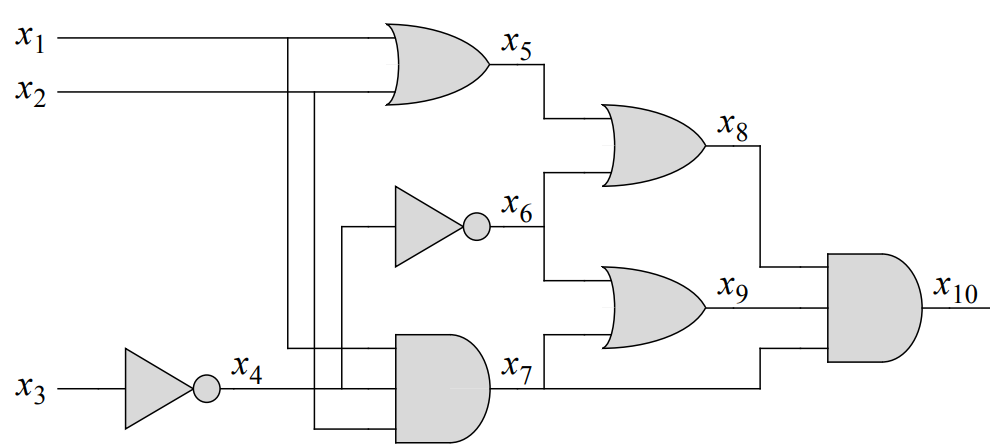
\includegraphics[scale=0.3]{imgs/circuit.png}
\end{figure}
Expresión \(\varphi\)
\begin{align*}
    \varphi = x_{10} &\land \left(x_{4} \longleftrightarrow \neg x_{3} \right) \\
                     &\land \left(x_{5} \longleftrightarrow \left(x_{1} \lor x_{2} \right) \right) \\
                     &\land \left(x_{6} \longleftrightarrow \neg x_{4} \right) \\
                     &\land \left(x_{7} \longleftrightarrow \left(x_{1} \land x_{2} \land x_{4} \right) \right) \\
                     &\land \left(x_{8} \longleftrightarrow \left(x_{5} \lor x_{6} \right) \right) \\
                     &\land \left(x_{9} \longleftrightarrow \left(x_{6} \lor x_{7} \right) \right) \\
                     &\land \left(x_{10} \longleftrightarrow \left(x_{7} \land x_{8} \land x_{9} \right) \right) \\
\end{align*}
\subsection{Algoritmo}
Sea \(\varphi\) un ejemplar genérico de \(3-\mathbf{CNF}-\mathbf{SAT}\).
\begin{itemize}
    \item Fase adivinadora:
    \begin{itemize}
        \item Para cada variable \(x_{i}\) con \(i \in \{1, 2, \dotsc, n\}\) le asignamos de manera arbitraria una constante lógica 
        \textit{(las constantes lógicas están dadas por el conjunto \(\{0, 1\}\) donde \(0\) es \texttt{Falso} y \(1\) es \texttt{Verdadero})}.
        Así hemos formado una asignación de valor para todas las variables que aparecen en las \(m\) cláusulas de la expresión lógica \(\varphi\)
    \end{itemize}
    \item Fase verificadora:
    \begin{itemize}
        \item Para cada cláusula \(m\) de \(\varphi\) evaluamos a \(m\) mediante sus variables cuyo valor se les dió en la \textbf{fase adivinadora},
        y una vez que hemos evaluado a toda cláusula \(m\) debemos de evaluar con esos valores la expresión lógica \(\varphi\).
        \item Sí \(\varphi \equiv 1\) entonces \(\varphi\) es satisfacible, en el otro caso \(\varphi\) es no satisfacible.
    \end{itemize}
\end{itemize}
\subsection{Técnica para la demostración del problema}
\noindent
Reemplazo local
\subsection{Aplicación en la vida real}
\begin{itemize}
    \item Pruebas automáticas para circuitos.
    \item Manejo de paquetes.
    \item Biología computacional.
    \item Física de partículas.
    \item Criptoanálisis.
    \item Resolución de muchos problemas en teoría de gráficas.
\end{itemize}
\newpage
\section{3-CNF-SAT}
\subsection{Definiciones previas}
\subsubsection{Literal}
\noindent
Una literal en una expresión lógica es una variable lógica o la negación de esa variable lógica.
\subsubsection{Forma Normal Conjuntiva}
\noindent
Una expresión lógica está en \textbf{Forma Normal Conjuntiva} sí ésta está expresada como una 
conjunción de cláusulas lógicas, a su vez cada una de éstas cláusulas son disyunciones de una 
o más literales.
\subsubsection{3-Forma Normal Conjuntiva}
\noindent
Una expresión lógica está en \textbf{3-forma normal conjuntiva} o \textbf{3-FNC} sí cada cláusula tiene
exactamente tres literales distintas. 
\newline 
\textbf{Ejemplo}
\[
    \left(x_{1} \lor \neg x_{1} \lor \neg x_{2}\right) \land \left(x_{3} \lor x_{2} \lor x_{4}\right) \land \left(\neg x_{1} \lor \neg x_{3} \lor x_{4}\right)
\]
es una expresión lógica en \textbf{3-FNC}.
\newline 
La primera cláusula de la expresión lógica \(\left(x_{1} \lor \neg x_{1} \lor \neg x_{2}\right)\), contiene exactamente \(3\) literales, las 
cuales son:
\begin{itemize}
    \item \(x_{1}\)
    \item \(\neg x_{1}\)
    \item \(\neg x_{2}\)
\end{itemize}
\subsection{Forma canónica o estándar}
\subsubsection{Ejemplar genérico}
\noindent
Una expresión lógica \(\varphi\) en \textbf{3-FNC}
\subsubsection{Pregunta de decisión}
\noindent
La expresión lógica \(\varphi\) ¿es satisfacible?
\subsection{Ejemplo}
\noindent
Consideremos la siguiente expresión lógica \(\varphi\)
\[
    \varphi = \left(x_{1} \lor x_{2} \lor \neg x_{3}\right) \land \left(\neg x_{1} \lor \neg x_{2} \lor x_{3}\right) \land \left(x_{1} \lor \neg x_{2} \lor x_{3}\right)
\]
\(\varphi\) es satisfacible ya que existe la siguiente asignación \(\langle x_{1} = 0, x_{2} = 0, x_{3} = 0 \rangle\)
\begin{align*}
    \varphi &= \left(0 \lor 0 \lor \neg 0\right) \land \left(\neg 0 \lor \neg 0 \lor 0\right) \land \left(0 \lor \neg 0 \lor 0\right) \\
            &= \left(0 \lor 0 \lor 1\right) \land \left(\neg 0 \lor \neg 0 \lor 0\right) \land \left(0 \lor \neg 0 \lor 0\right) \\
            &= \left(0 \lor 0 \lor 1\right) \land \left(1 \lor 1 \lor 0\right) \land \left(0 \lor \neg 0 \lor 0\right) \\
            &= \left(0 \lor 0 \lor 1\right) \land \left(1 \lor 1 \lor 0\right) \land \left(0 \lor 1 \lor 0\right) \\
            &= \left(1\right) \land \left(1\right) \land \left(1\right) \\
            &= 1
\end{align*}
\subsection{Teorema}
\noindent
El problema \textbf{3-CNF-SAT} es \textbf{NP-}Completo.
\newpage
\subsection{Demostración}
\noindent
Iniciaremos mostrando que el problema \textbf{3-CNF-SAT} pertence a la clase \(\mathbf{NP}\). 
\newline 
Tenemos que dar un algoritmo que verifique que una expresión lógica en \textbf{3-FNC} \(\varphi\) es satisfacible dada una 
asignación de valor a las variables. El algoritmo es muy sencillo, simplemente sustituimos cada variable 
por su valor correspondiente y evaluamos la expresión, exactamente como se hizo en el ejemplo. Notemos que 
éste algoritmo está dado en tiempo \(O\left(m\right)\) ya que el número de literales de cada cláusula permanece constante, 
ya que siempre es \(3\).
\subsubsection{Transformación}
\noindent
Transformaremos un ejemplar genérico del problema \textbf{SAT} en un ejemplar genérico de \textbf{3-CNF-SAT}.
\newline 
La transformación se realizará en \(3\) pasos.
\newline 
\textbf{Paso 1}
\newline
Sea \(\varphi\) la expresión lógica que es el ejemplar genérico del problema \textbf{SAT}, construiremos un árbol binario 
para la fórmulta \(\varphi\), las literales serán las hojas del árbol, mientras que los operadores lógicos \textit{(recordemos que en 
el problema \textbf{SAT} los operadores lógicos pueden ser distintos a \(\land, \lor\) y \(\neg\))}.
\newline 
Sí la fórmuta contiene una cláusula tal que ésta cláusula es la \textbf{disyunción} de varias literales entonces usamos la asocitividad de 
la disyunción para agregar paréntesis a la expresión, con ésto logramos que cada nodo interno tenga uno o dos nodos hijos. 
\newline 
\textbf{Introducción de nuevas variables}
\newline 
Crearemos nuevas variables \(y_{i}\) por cada nodo interno del árbol binario creado.
\newline 
\textbf{Operaciones en nodos del árbol}
\newline 
Sea \(y_{i}\) una nueva variable introducida en un nodo interno del árbol y sea \(\diamond\) un operador lógico tal que 
\(\diamond \in \{\land, \lor, \longleftarrow, \longleftrightarrow \}\) y \(\diamond\) está en el nodo interno del árbol.
Tenemos tres casos para los nodos hijos de \(y_{i}\):
\begin{enumerate}
    \item Ambos nodos hijos de \(y_{i}\) son nodos internos, los cuales a su vez le fueron introducidos nuevas variables las cuales denotaremos como \(y_{j}\) y \(y_{k}\).
    \item Uno de los nodos hijos de \(y_{i}\) es un nodo interno mientras que el otro es una hoja, el nodo interno será denotado como \(y_{k}\) y la literal correspondiente a la hoja será denotada como \(x_{n}\).
    \item Ambos nodos hijos de \(y_{i}\) son hojas, las literales correspondientes a la hojas serán denotadas como \(x_{n}\) y \(x_{m}\).
\end{enumerate}
El primer nodo mencionado en los casos anteriores será tomado como el hijo izquierdo de \(y_{i}\) mientras que el último será tomado como el hijo derecho de \(y_{i}\).
\newline
Para la operación en algún nodo interno \(y_{i}\) tenemos tres casos:
\newline
Caso (1)
\newline 
\(y_{i} \longleftrightarrow \left(y_{j} \diamond y_{k}\right)\)
\newline 
Caso (2)
\newline 
\(y_{i} \longleftrightarrow \left(y_{k} \diamond x_{n}\right)\)
\newline 
Caso (3)
\newline 
\(y_{i} \longleftrightarrow \left(x_{n} \diamond x_{m}\right)\)
\newline 
Notemos que siempre se pone primero el nodo hijo izquierdo y después el nodo hijo derecho, esto siempre se hace así por el operador lógico \(\longrightarrow\) ya que no es 
lo mismo \(p \longrightarrow q\) que \(q \longrightarrow p\). 
\newline 
Para los casos simétricos de los casos mencionados se hace exactamente lo mismo, respetando el orden que definimos en el párrafo anterior.
\newline
Cuando el operador lógico es \(\neg\) sólo tenemos dos casos ya que solemante tenemos un nodo hijo para \(y_{i}\):
\begin{enumerate}
    \item El nodo hijo de \(y_{i}\) es un nodo interno, el nodo interno será denotado como \(y_{k}\).
    \item El nodo hijo de \(y_{i}\) es una hoja, la hora será denotada como \(x_{n}\).
\end{enumerate}
Para la operación en algún nodo interno \(y_{i}\) tenemos 2 casos:
\newline
Caso (1)
\newline 
\(y_{i} \longleftrightarrow \neg y_{k}\)
\newline 
Caso (2)
\newline 
\(y_{i} \longleftrightarrow \neg x_{n}\)
\newline 
Reescribiremos la expresión lógica original \(\varphi\) como una conjunción de la variable que está en la raíz del árbol y una conjunción 
de cláusulas que describe las operaciones en cada nodo \textit{(éstas operaciones ya han sido descritas y cubiertas en todos su casos)}, 
a ésta reescritura de la expresión lógica \(\varphi\) la denotaremos como \(\varphi'\).
\newline
Por como definimos cada operación en un nodo interno, notemos que la expresión lógica \(\varphi'\) es una conjunción de cláusulas y además de ésto
cada cláusula tiene a lo más tres literales \textit{(ésto debido al operador lógico \(\neg\))}.
\newline 
\textbf{Segundo paso}.
\newline 
Convertiremos cada cláusula de la expresión lógica \(\varphi'\) en \textbf{forma normal conjuntiva}. Para cada cláusula \(c\) de la expresión 
lógica \(\varphi'\) construiremos su tabla de verdad, usando las entradas para las literales de la tabla de verdad que hacen que la cláusula \(c\)
se evalúen a \(0\), construiremos la expresión en \textbf{Forma Normal Disjuntiva} \textit(una disyunción de conjunciones) notemos que ésto es equivalente a 
\(\neg c\), ya que tomaremos como verdaderas precisamente esos renglones donde sea hace \(0\) \(c\), una vez que tenemos una disyunción de conjunciones negaremos 
ésta cláusula para tener una equivalente a la cláusula \(c\), ya que recordemos que \(\neg \neg c \equiv c\), y por las \textbf{leyes de DeMorgan} nos 
quedará la cláusula en \textbf{forma normal conjuntiva}. En éste punto hemos puesto cada cláusula \(c\) de \(\varphi'\) en \textbf{Forma Normal Conjuntiva}
y por como construimos \(\varphi'\) ahora ésta también está en \textbf{Forma Normal Conjuntiva}, a ésta última expresión lógica la denotaremos como \(\varphi''\).
Así todas las cláusulas de \(\varphi''\) están en \textbf{forma normal conjuntiva} y cada cláusula tiene a los \(3\) literales.
\newline 
\textbf{Tercer paso}
\newline 
Haremos que cada cláusula de la expresión lógica \(\varphi''\) tenga exactamente \(3\) literales. Construiremos una expresión lógica
\(\varphi'''\) a partir de las cláusulas de la expresión lógica \(\varphi''\). La expresión lógica \(\varphi'''\) hará usó de dos nuevas 
literales las cuales llamaremos \(p\) y \(q\). Lo que se hará es lo siguiente:
Sea \(C\) una cláusula de la expresión lógica \(\varphi''\), incluiremos las siguientes cláusulas en \(\varphi'''\):
\begin{itemize}
    \item Sí \(C\) tiene exactamente \(3\) literales distintas entonces incluimos a \(C\) tal como está en \(\varphi'''\)
    \item Sí \(C\) tiene \(2\) literales distintas entonces \(C = l_{1} \lor l_{2}\), entonces incluiremos en \(\varphi'''\)
          las cláusulas \(l_{1} \lor l_{2} \lor p\) y \(l_{1} \lor l_{2} \lor  \neg p\). Notemos que ésto no afecta a la fórmula 
          original \(\varphi''\) ya que independiente del valor \(p\) al evaluarlo una cláusula nos dará \(l_{1} \lor l_{2}\) y la otra 
          nos dará \(1\) y sabemos que siempre se cumple que \(\left(l_{1} \lor l_{2}\right) \land 1 \equiv l_{1} \lor l_{2}\).
    \item Sí \(C\) tiene \(1\) literal distinta entonces \(C = l_{1}\), entonces incluiremos en \(\varphi'''\)
          las cláusulas \(l_{1} \lor l_{2} \lor p \lor q\), \(l_{1} \lor l_{2} \lor \neg p \lor q\), \(l_{1} \lor l_{2} \lor p \lor \neg q\) 
          y \(l_{1} \lor l_{2} \lor \neg p \lor \neg q\). Notemos que ésto no afecta a la fórmula original \(\varphi''\) ya que 
          independiente del valor de \(p\) y \(q\) al evaluarlo una cláusula nos dará \(l_{1}\) y las otras nos dará \(1\) y 
          sabemos que siempre se cumple que \(l_{1} \land 1 \land 1 \land 1 \equiv l_{1}\).
\end{itemize}
\subsubsection{Afirmación}
\noindent
\(\varphi\) es satisfacible sí y sólo sí \(\varphi'''\) es satisfacible.
\newline 
Notemos que por construcción de \(\varphi'\) en el primer paso ésta es equivalente a \(\varphi\),
ya que el operador \(\longleftrightarrow\), también notemos que que en el segundo paso lo único 
que se hizo fue poner a \(\varphi'\) en \textbf{forma normal conjuntiva} y finalmente en el tercer paso
mostramos que no importaba sí le agregamos literales a las cláusulas ya que éstas preservan el significa original
a la expresión lógica \(\varphi''\), por lo tanto \(\varphi'''\) es equivalente a \(\varphi''\), por lo tanto tenemos que 
\[
    \varphi \longleftrightarrow \varphi' \longleftrightarrow \varphi'' \longleftrightarrow \varphi'''
\]
De lo que se sigue que
\[
    \varphi \longleftrightarrow \varphi'''
\]
\newpage
\subsection{Ejemplificación de la transformación}
\noindent
\[
    \varphi = \left(\left(x_{1} \longrightarrow x_{2}\right) \lor \neg \left(\left(\neg x_{1} \longleftrightarrow x_{3}\right) \lor x_{4}\right)\right) \land \neg x_{2}
\]
\textbf{Primer Paso}
\newline 
Construcción del \textbf{árbol binario}.
\newline
\begin{figure}[H]
    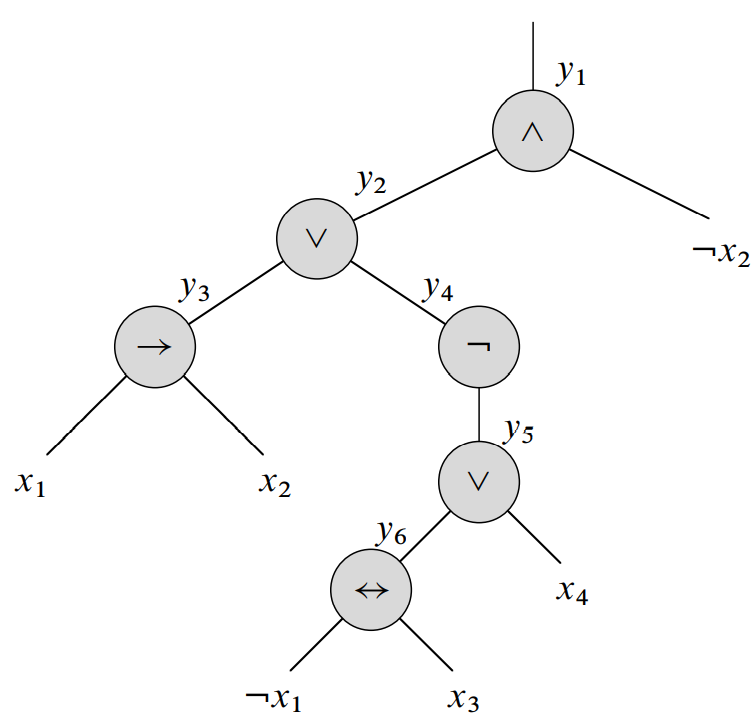
\includegraphics[scale=0.3]{imgs/binary_tree.png}
\end{figure}
Construcción de \(\varphi'\)
\begin{align*}
    \varphi = y_{1} &\land \left(y_{1} \longleftrightarrow \left(y_{2} \land \neg x_{2}\right)\right) \\
                    &\land \left(y_{2} \longleftrightarrow \left(y_{3} \lor y_{4}\right)\right) \\
                    &\land \left(y_{3} \longleftrightarrow \left(x_{1} \longrightarrow x_{2}\right)\right) \\
                    &\land \left(y_{4} \longleftrightarrow \neg y_{5}\right) \\
                    &\land \left(y_{5} \longleftrightarrow \left(y_{6} \lor x_{4}\right)\right) \\
                    &\land \left(y_{6} \longleftrightarrow \left(\neg x_{1} \longleftrightarrow x_{3}\right)\right)
\end{align*}
\textbf{Segundo Paso}
\textbf{Segundo Paso}
\newline 
Construcción de tablas de verdad por cada cláusula
\newline 
\(y_1\)
\newline 
\begin{tabular}{@{ }c | c}
    \(y_{1}\) & \(y_{1}\)\\
    \hline 
    1 & \textcolor{red}{1}\\
    0 & \textcolor{red}{0}\\
\end{tabular}
\newline
\(y_{1} \longleftrightarrow \left(y_{2} \land \neg x_{2}\right)\)
\newline
\begin{tabular}{@{ }c@{ }@{ }c@{ }@{ }c | c@{ }@{ }c@{ }@{ }c@{ }@{}c@{}@{ }c@{ }@{ }c@{ }@{ }c@{ }@{ }c@{ }@{}c@{}@{ }c}
    \(y_{1}\) & \(y_{2}\) & \(x_{2}\) &  & \(y_{1}\) & $\leftrightarrow$ & ( & \(y_{2}\) & $\land$ & $\lnot$ & \(x_{2}\) & ) & \\
    \hline 
    1 & 1 & 1 &  & 1 & \textcolor{red}{0} &  & 1 & 0 & 0 & 1 &  & \\
    1 & 1 & 0 &  & 1 & \textcolor{red}{1} &  & 1 & 1 & 1 & 0 &  & \\
    1 & 0 & 1 &  & 1 & \textcolor{red}{0} &  & 0 & 0 & 0 & 1 &  & \\
    1 & 0 & 0 &  & 1 & \textcolor{red}{0} &  & 0 & 0 & 1 & 0 &  & \\
    0 & 1 & 1 &  & 0 & \textcolor{red}{1} &  & 1 & 0 & 0 & 1 &  & \\
    0 & 1 & 0 &  & 0 & \textcolor{red}{0} &  & 1 & 1 & 1 & 0 &  & \\
    0 & 0 & 1 &  & 0 & \textcolor{red}{1} &  & 0 & 0 & 0 & 1 &  & \\
    0 & 0 & 0 &  & 0 & \textcolor{red}{1} &  & 0 & 0 & 1 & 0 &  & \\
\end{tabular}
\newline
\textbf{Forma Normal Disjuntiva}
\[
    \left(y_{1} \land y_{2} \land x_{2}\right) \lor \left(y_{1} \land \neg y_{2} \land x_{2}\right) \lor 
    \left(y_{1} \land \neg y_{2} \land \neg x_{2}\right) \lor \left(\neg y_{1} \land y_{2} \land \neg x_{2}\right)
\]
\textbf{De Morgan}
\[
    \left(\neg y_{1} \lor \neg y_{2} \lor \neg x_{2}\right) \land \left( \neg y_{1} \lor y_{2} \lor \neg x_{2}\right) \land
    \left(\neg y_{1} \lor y_{2} \lor x_{2}\right) \land \left( y_{1} \lor \neg y_{2} \lor x_{2}\right)
\]
\textbf{Forma Normal Conjuntiva}
\[
    \left(\neg y_{1} \lor \neg y_{2} \lor \neg x_{2}\right) \land \left( \neg y_{1} \lor y_{2} \lor \neg x_{2}\right) \land
    \left(\neg y_{1} \lor y_{2} \lor x_{2}\right) \land \left( y_{1} \lor \neg y_{2} \lor x_{2}\right) % Ya agregado
\]
\newpage
\(y_{2} \longleftrightarrow \left(y_{3} \lor y_{4}\right)\)
\newline
\begin{tabular}{@{ }c@{ }@{ }c@{ }@{ }c | c@{ }@{ }c@{ }@{ }c@{ }@{}c@{}@{ }c@{ }@{ }c@{ }@{ }c@{ }@{}c@{}@{ }c}
    \(y_{2}\) & \(y_{3}\) & \(y_{4}\) &  & \(y_{2}\) & $\leftrightarrow$ & ( & \(y_{3}\) & $\lor$ & \(y_{4}\) & ) & \\
    \hline 
    1 & 1 & 1 &  & 1 & \textcolor{red}{1} &  & 1 & 1 & 1 &  & \\
    1 & 1 & 0 &  & 1 & \textcolor{red}{1} &  & 1 & 1 & 0 &  & \\
    1 & 0 & 1 &  & 1 & \textcolor{red}{1} &  & 0 & 1 & 1 &  & \\
    1 & 0 & 0 &  & 1 & \textcolor{red}{0} &  & 0 & 0 & 0 &  & \\
    0 & 1 & 1 &  & 0 & \textcolor{red}{0} &  & 1 & 1 & 1 &  & \\
    0 & 1 & 0 &  & 0 & \textcolor{red}{0} &  & 1 & 1 & 0 &  & \\
    0 & 0 & 1 &  & 0 & \textcolor{red}{0} &  & 0 & 1 & 1 &  & \\
    0 & 0 & 0 &  & 0 & \textcolor{red}{1} &  & 0 & 0 & 0 &  & \\
\end{tabular}
\newline
\textbf{Forma Normal Disjuntiva}
\[
    \left(y_{2} \land \neg y_{3} \land \neg y_{4}\right) \lor \left(\neg y_{2} \land y_{3} \land y_{4}\right) \lor 
    \left(\neg y_{2} \land y_{3} \land \neg y_{4}\right) \lor \left(\neg y_{2} \land \neg y_{3} \land y_{4} \right)
\]
\textbf{De Morgan}
\[
    \neg \left(\left(y_{2} \land \neg y_{3} \land \neg y_{4}\right) \lor \left(\neg y_{2} \land y_{3} \land y_{4}\right) \lor 
    \left(\neg y_{2} \land y_{3} \land \neg y_{4}\right) \lor \left(\neg y_{2} \land \neg y_{3} \land y_{4} \right)\right)
\]
equivalente a
\[
    \neg \left(y_{2} \land \neg y_{3} \land \neg y_{4}\right) \land \neg \left(\neg y_{2} \land y_{3} \land y_{4}\right) \land
    \neg \left(\neg y_{2} \land y_{3} \land \neg y_{4}\right) \land \neg \left(\neg y_{2} \land \neg y_{3} \land y_{4} \right)
\]
equivalente a
\[
    \left( \neg y_{2} \lor  \neg\neg y_{3} \lor \neg\neg y_{4}\right) \land \left(\neg\neg y_{2} \land \neg y_{3} \land \neg y_{4}\right) \land
    \left(\neg \neg y_{2} \lor  \neg y_{3} \lor  \neg\neg y_{4}\right) \land \left(\neg\neg y_{2} \lor \neg\neg y_{3} \lor \neg y_{4} \right)
\]
equivalente a
\[
    \left( \neg y_{2} \lor y_{3} \lor y_{4}\right) \land \left(y_{2} \land \neg y_{3} \land \neg y_{4}\right) \land
    \left(y_{2} \lor  \neg y_{3} \lor  y_{4}\right) \land \left(y_{2} \lor y_{3} \lor \neg y_{4} \right)
\]
\textbf{Forma Normal Conjuntiva}
\[
    \left( \neg y_{2} \lor y_{3} \lor y_{4}\right) \land \left(y_{2} \land \neg y_{3} \land \neg y_{4}\right) \land
    \left(y_{2} \lor  \neg y_{3} \lor  y_{4}\right) \land \left(y_{2} \lor y_{3} \lor \neg y_{4} \right) % Ya agregado
\]
\(y_{3} \longleftrightarrow \left(x_{1} \longrightarrow x_{2}\right)\)
\newline
\begin{tabular}{@{ }c@{ }@{ }c@{ }@{ }c | c@{ }@{ }c@{ }@{ }c@{ }@{}c@{}@{ }c@{ }@{ }c@{ }@{ }c@{ }@{}c@{}@{ }c}
    \(y_{3}\) & \(x_{1}\) & \(x_{2}\) &  & \(y_{3}\) & $\leftrightarrow$ & ( & \(x_{1}\) & $\rightarrow$ & \(x_{2}\) & ) & \\
    \hline 
    1 & 1 & 1 &  & 1 & \textcolor{red}{1} &  & 1 & 1 & 1 &  & \\
    1 & 1 & 0 &  & 1 & \textcolor{red}{0} &  & 1 & 0 & 0 &  & \\
    1 & 0 & 1 &  & 1 & \textcolor{red}{1} &  & 0 & 1 & 1 &  & \\
    1 & 0 & 0 &  & 1 & \textcolor{red}{1} &  & 0 & 1 & 0 &  & \\
    0 & 1 & 1 &  & 0 & \textcolor{red}{0} &  & 1 & 1 & 1 &  & \\
    0 & 1 & 0 &  & 0 & \textcolor{red}{1} &  & 1 & 0 & 0 &  & \\
    0 & 0 & 1 &  & 0 & \textcolor{red}{0} &  & 0 & 1 & 1 &  & \\
    0 & 0 & 0 &  & 0 & \textcolor{red}{0} &  & 0 & 1 & 0 &  & \\
\end{tabular}
\newline
\textbf{Forma Normal Disjuntiva}
\newline
\[
    \left(y_{3} \land x_{1} \land \neg x_{2}\right) \lor \left(\neg y_{3} \land x_{1} \land x_{2}\right) \lor
    \left(\neg y_{3} \land \neg x_{1} \land x_{2}\right) \lor \left(\neg y_{3} \land \neg x_{1} \land \neg x_{2}\right)
\]
\textbf{De Morgan}
\[
    \neg \left(\left(y_{3} \land x_{1} \land \neg x_{2}\right) \lor \left(\neg y_{3} \land x_{1} \land x_{2}\right) \lor
    \left(\neg y_{3} \land \neg x_{1} \land x_{2}\right) \lor \left(\neg y_{3} \land \neg x_{1} \land \neg x_{2}\right)\right)
\]
equivalente a
\[
    \neg \left(y_{3} \land x_{1} \land \neg x_{2}\right) \land \neg \left(\neg y_{3} \land x_{1} \land x_{2}\right) \land
    \neg \left(\neg y_{3} \land \neg x_{1} \land x_{2}\right) \land \neg \left(\neg y_{3} \land \neg x_{1} \land \neg x_{2}\right)
\]
equivalente a
\[
    \left(\neg y_{3} \lor \neg x_{1} \lor \neg \neg x_{2}\right) \land \left(\neg \neg y_{3} \lor \neg x_{1} \lor \neg x_{2}\right) \land
    \left(\neg \neg y_{3} \lor \neg \neg x_{1} \lor \neg x_{2}\right) \land \left(\neg \neg y_{3} \lor \neg \neg x_{1} \lor \neg \neg x_{2}\right)
\]
equivalente a
\[
    \left(\neg y_{3} \lor \neg x_{1} \lor x_{2}\right) \land \left(y_{3} \lor \neg x_{1} \lor \neg x_{2}\right) \land
    \left(y_{3} \lor x_{1} \lor \neg x_{2}\right) \land \left(y_{3} \lor x_{1} \lor x_{2}\right)
\]
\textbf{Forma Normal Conjuntiva}
\[
    \left(\neg y_{3} \lor \neg x_{1} \lor x_{2}\right) \land \left(y_{3} \lor \neg x_{1} \lor \neg x_{2}\right) \land
    \left(y_{3} \lor x_{1} \lor \neg x_{2}\right) \land \left(y_{3} \lor x_{1} \lor x_{2}\right) % Ya agregado
\]
\(y_{4} \longleftrightarrow \neg y_{5}\)
\newline
\begin{tabular}{@{ }c@{ }@{ }c | c@{ }@{ }c@{ }@{ }c@{ }@{ }c@{ }@{ }c@{ }@{ }c}
    \(y_{4}\) & \(y_{5}\) &  & \(y_{4}\) & $\leftrightarrow$ & $\lnot$ & \(y_{5}\) & \\
    \hline 
    1 & 1 &  & 1 & \textcolor{red}{0} & 0 & 1 & \\
    1 & 0 &  & 1 & \textcolor{red}{1} & 1 & 0 & \\
    0 & 1 &  & 0 & \textcolor{red}{1} & 0 & 1 & \\
    0 & 0 &  & 0 & \textcolor{red}{0} & 1 & 0 & \\
\end{tabular}
\newline
\textbf{Forma Normal Disjuntiva}
\[
    \left(y_{4} \land y_{5}\right) \lor \left(\neg y_{4} \land \neg y_{5}\right)
\]
\textbf{De Morgan}
\[
    \neg \left(\left(y_{4} \land y_{5}\right) \lor \left(\neg y_{4} \land \neg y_{5}\right)\right)
\]
equivalente a
\[
    \neg \left(y_{4} \land y_{5}\right) \land \neg \left(\neg y_{4} \land \neg y_{5}\right)
\]
equivalente a
\[
    \left(\neg y_{4} \lor \neg y_{5}\right) \land \left(\neg \neg y_{4} \lor \neg \neg y_{5}\right)
\]
equivalente a
\[
    \left(\neg y_{4} \lor \neg y_{5}\right) \land \left(y_{4} \lor y_{5}\right)
\]
\textbf{Forma Normal Conjuntiva}
\[
    \left(\neg y_{4} \lor \neg y_{5}\right) \land \left(y_{4} \lor y_{5}\right) % Ya agregado
\]
\(y_{5} \longleftrightarrow \left(y_{6} \lor x_{4}\right)\)
\newline
\begin{tabular}{@{ }c@{ }@{ }c@{ }@{ }c | c@{ }@{ }c@{ }@{ }c@{ }@{}c@{}@{ }c@{ }@{ }c@{ }@{ }c@{ }@{}c@{}@{ }c}
    \(y_{5}\) & \(y_{6}\) & \(x_{4}\) &  & \(y_{5}\) & $\leftrightarrow$ & ( & \(y_{6}\) & $\lor$ & \(x_{4}\) & ) & \\
    \hline 
    1 & 1 & 1 &  & 1 & \textcolor{red}{1} &  & 1 & 1 & 1 &  & \\
    1 & 1 & 0 &  & 1 & \textcolor{red}{1} &  & 1 & 1 & 0 &  & \\
    1 & 0 & 1 &  & 1 & \textcolor{red}{1} &  & 0 & 1 & 1 &  & \\
    1 & 0 & 0 &  & 1 & \textcolor{red}{0} &  & 0 & 0 & 0 &  & \\
    0 & 1 & 1 &  & 0 & \textcolor{red}{0} &  & 1 & 1 & 1 &  & \\
    0 & 1 & 0 &  & 0 & \textcolor{red}{0} &  & 1 & 1 & 0 &  & \\
    0 & 0 & 1 &  & 0 & \textcolor{red}{0} &  & 0 & 1 & 1 &  & \\
    0 & 0 & 0 &  & 0 & \textcolor{red}{1} &  & 0 & 0 & 0 &  & \\
\end{tabular}
\newline
\textbf{Forma Normal Disjuntiva}
\[
    \left(y_{5} \land \neg y_{6} \land \neg x_{4}\right) \lor \left(\neg y_{5} \land y_{6} \land x_{4}\right) \lor
    \left(\neg y_{5} \land y_{6} \land \neg x_{4} \right) \lor \left(\neg y_{5} \land \neg y_{6} \land x_{4}\right)
\]
\textbf{De Morgan}
\[
    \neg \left(\left(y_{5} \land \neg y_{6} \land \neg x_{4}\right) \lor \left(\neg y_{5} \land y_{6} \land x_{4}\right) \lor
    \left(\neg y_{5} \land y_{6} \land \neg x_{4} \right) \lor \left(\neg y_{5} \land \neg y_{6} \land x_{4}\right)\right)
\]
equivalente a
\[
    \neg \left(y_{5} \land \neg y_{6} \land \neg x_{4}\right) \land \neg \left(\neg y_{5} \land y_{6} \land x_{4}\right) \land
    \neg \left(\neg y_{5} \land y_{6} \land \neg x_{4} \right) \land \neg \left(\neg y_{5} \land \neg y_{6} \land x_{4}\right)
\]
equivalente a
\[
    \left(\neg y_{5} \lor \neg \neg y_{6} \lor \neg \neg x_{4}\right) \land \left(\neg \neg y_{5} \lor \neg y_{6} \lor \neg x_{4}\right) \land
    \left(\neg \neg y_{5} \lor \neg y_{6} \lor \neg \neg x_{4} \right) \land \left(\neg \neg y_{5} \lor \neg \neg y_{6} \lor \neg x_{4}\right)
\]
equivalente a
\[
    \left(\neg y_{5} \lor y_{6} \lor x_{4}\right) \land \left(y_{5} \lor \neg y_{6} \lor \neg x_{4}\right) \land
    \left(y_{5} \lor \neg y_{6} \lor x_{4} \right) \land \left(y_{5} \lor y_{6} \lor \neg x_{4}\right)
\]
\textbf{Forma Normal Conjuntiva}
\[
    \left(\neg y_{5} \lor y_{6} \lor x_{4}\right) \land \left(y_{5} \lor \neg y_{6} \lor \neg x_{4}\right) \land
    \left(y_{5} \lor \neg y_{6} \lor x_{4} \right) \land \left(y_{5} \lor y_{6} \lor \neg x_{4}\right) % Ya agregado 
\]
\newpage
\(y_{6} \longleftrightarrow \left(\neg x_{1} \longleftrightarrow x_{3}\right)\)
\newline
\begin{tabular}{@{ }c@{ }@{ }c@{ }@{ }c | c@{ }@{ }c@{ }@{ }c@{ }@{}c@{}@{ }c@{ }@{ }c@{ }@{ }c@{ }@{ }c@{ }@{}c@{}@{ }c}
    \(y_{6}\) & \(x_{1}\) & \(x_{3}\) &  & \(y_{6}\) & $\leftrightarrow$ & ( & $\lnot$ & \(x_{1}\) & $\leftrightarrow$ & \(x_{3}\) & ) & \\
    \hline 
    1 & 1 & 1 &  & 1 & \textcolor{red}{0} &  & 0 & 1 & 0 & 1 &  & \\
    1 & 1 & 0 &  & 1 & \textcolor{red}{1} &  & 0 & 1 & 1 & 0 &  & \\
    1 & 0 & 1 &  & 1 & \textcolor{red}{1} &  & 1 & 0 & 1 & 1 &  & \\
    1 & 0 & 0 &  & 1 & \textcolor{red}{0} &  & 1 & 0 & 0 & 0 &  & \\
    0 & 1 & 1 &  & 0 & \textcolor{red}{1} &  & 0 & 1 & 0 & 1 &  & \\
    0 & 1 & 0 &  & 0 & \textcolor{red}{0} &  & 0 & 1 & 1 & 0 &  & \\
    0 & 0 & 1 &  & 0 & \textcolor{red}{0} &  & 1 & 0 & 1 & 1 &  & \\
    0 & 0 & 0 &  & 0 & \textcolor{red}{1} &  & 1 & 0 & 0 & 0 &  & \\
\end{tabular}
\newline
\textbf{Forma Normal Disjuntiva}
\[
    \left(y_{6} \land x_{1} \land x_{3}\right) \lor \left(y_{6} \land \neg x_{1} \land \neg x_{3}\right) \lor
    \left(\neg y_{6} \land x_{1} \land \neg x_{3}\right) \lor \left(\neg y_{6} \land \neg x_{1} \land x_{3}\right)
\]
\textbf{De Morgan}
\[
    \neg \left(\left(y_{6} \land x_{1} \land x_{3}\right) \lor \left(y_{6} \land \neg x_{1} \land \neg x_{3}\right) \lor
    \left(\neg y_{6} \land x_{1} \land \neg x_{3}\right) \lor \left(\neg y_{6} \land \neg x_{1} \land x_{3}\right)\right)
\]
equivalente a
\[
    \neg \left(y_{6} \land x_{1} \land x_{3}\right) \land \neg \left(y_{6} \land \neg x_{1} \land \neg x_{3}\right) \land
    \neg \left(\neg y_{6} \land x_{1} \land \neg x_{3}\right) \land \neg \left(\neg y_{6} \land \neg x_{1} \land x_{3}\right)
\]
equivalente a
\[
    \left(\neg y_{6} \lor \neg x_{1} \lor \neg x_{3}\right) \land \left(\neg y_{6} \lor \neg \neg x_{1} \lor \neg \neg x_{3}\right) \land
    \left(\neg \neg y_{6} \lor \neg x_{1} \lor \neg \neg x_{3}\right) \land \left(\neg \neg y_{6} \lor \neg \neg x_{1} \lor \neg x_{3}\right)
\]
equivalente a
\[
    \left(\neg y_{6} \lor \neg x_{1} \lor \neg x_{3}\right) \land \left(\neg y_{6} \lor x_{1} \lor x_{3}\right) \land
    \left(y_{6} \lor \neg x_{1} \lor x_{3}\right) \land \left(y_{6} \lor x_{1} \lor \neg x_{3}\right)
\]
\textbf{Forma Normal Conjuntiva}
\[
    \left(\neg y_{6} \lor \neg x_{1} \lor \neg x_{3}\right) \land \left(\neg y_{6} \lor x_{1} \lor x_{3}\right) \land
    \left(y_{6} \lor \neg x_{1} \lor x_{3}\right) \land \left(y_{6} \lor x_{1} \lor \neg x_{3}\right)
\]
\textbf{Tercer Paso}
\newline 
\textbf{Cláusulas que modificaremos para que tengan exactamente \(3\) literales}
\begin{itemize}
    \item \(y_{1}\)
    \item \(\neg y_{4} \lor \neg y_{5}\)
    \item \(\neg y_{4} \lor \neg y_{5}\)
\end{itemize}
\(y_{1}\) pasa a ser 
\[
    \left(y_{1} \lor p \lor q\right) \land \left(y_{1} \lor p \lor \neg q\right) \land \left(y_{1} \lor \neg p \lor q\right) \land \left(y_{1} \lor \neg p \lor \neg q\right)
\]
\(\neg y_{4} \lor \neg y_{5}\) pasa a ser 
\[
    \left(\neg y_{4} \lor \neg y_{5} \lor p\right) \land \left(\neg y_{4} \lor \neg y_{5} \lor \neg p\right)
\]
\(y_{4} \lor y_{5}\) pasa a ser 
\[
    \left(y_{4} \lor y_{5} \lor p\right) \land \left(y_{4} \lor y_{5} \lor \neg p\right)
\]
\textbf{Ejemplar genérico \(\varphi'''\) de} \(3-\mathbf{CNF-SAT}\)
\begin{align*}
    \varphi''' = \left(y_{1} \lor p \lor q\right) & \land \left(y_{1} \lor p \lor \neg q\right) \land \left(y_{1} \lor \neg p \lor q\right) \\
                & \land \left(y_{1} \lor \neg p \lor \neg q\right) \land \left(\neg y_{1} \lor \neg y_{2} \lor \neg x_{2}\right) \land \left( \neg y_{1} \lor y_{2} \lor \neg x_{2}\right) \\ 
                & \land \left(\neg y_{1} \lor y_{2} \lor x_{2}\right) \land \left( y_{1} \lor \neg y_{2} \lor x_{2}\right) \land \left( \neg y_{2} \lor y_{3} \lor y_{4}\right) \\ 
                & \land \left(y_{2} \land \neg y_{3} \land \neg y_{4}\right) \land \left(y_{2} \lor  \neg y_{3} \lor  y_{4}\right) \land \left(y_{2} \lor y_{3} \lor \neg y_{4} \right) \\
                & \land \left(\neg y_{3} \lor \neg x_{1} \lor x_{2}\right) \land \left(y_{3} \lor \neg x_{1} \lor \neg x_{2}\right) \land \left(y_{3} \lor x_{1} \lor \neg x_{2}\right) \\ 
                & \land \left(y_{3} \lor x_{1} \lor x_{2}\right) \land \left(\neg y_{4} \lor \neg y_{5} \lor p\right) \land \left(\neg y_{4} \lor \neg y_{5} \lor \neg p\right) \\
                & \land \left(y_{4} \lor y_{5} \lor p\right) \land \left(y_{4} \lor y_{5} \lor \neg p\right) \land \left(\neg y_{5} \lor y_{6} \lor x_{4}\right) \\
                & \land \left(y_{5} \lor \neg y_{6} \lor \neg x_{4}\right) \land \left(y_{5} \lor \neg y_{6} \lor x_{4} \right) \land \left(y_{5} \lor y_{6} \lor \neg x_{4}\right) \\ 
                & \land \left(\neg y_{6} \lor \neg x_{1} \lor \neg x_{3}\right) \land \left(\neg y_{6} \lor x_{1} \lor x_{3}\right) \land \left(y_{6} \lor \neg x_{1} \lor x_{3}\right) \\
                & \land \left(y_{6} \lor x_{1} \lor \neg x_{3}\right)
\end{align*}
\subsection{Algoritmo}
Sea \(\varphi\) un ejemplar genérico de \(3-\mathbf{CNF}-\mathbf{SAT}\).
\begin{itemize}
    \item Fase adivinadora:
    \begin{itemize}
        \item Para cada variable \(x_{i}\) con \(i \in \{1, 2, \dotsc, n\}\) le asignamos de manera arbitraria una constante lógica 
        \textit{(las constantes lógicas están dadas por el conjunto \(\{0, 1\}\) donde \(0\) es \texttt{Falso} y \(1\) es \texttt{Verdadero})}.
        Así hemos formado una asignación de valor para todas las variables que aparecen en las \(m\) cláusulas de la expresión lógica \(\varphi\)
    \end{itemize}
    \item Fase verificadora:
    \begin{itemize}
        \item Para cada cláusula \(m\) de \(\varphi\) evaluamos a \(m\) mediante sus variables cuyo valor se les dió en la \textbf{fase adivinadora},
        y una vez que hemos evaluado a toda cláusula \(m\) debemos de evaluar con esos valores la expresión lógica \(\varphi\).
        \item Sí \(\varphi \equiv 1\) entonces \(\varphi\) es satisfacible, en el otro caso \(\varphi\) es no satisfacible.
    \end{itemize}
\end{itemize}
\subsection{Técnica para la demostración del problema}
\noindent
Reemplazo local
\subsubsection{Aplicación en la vida real}
\begin{itemize}
    \item Pruebas automáticas para circuitos.
    \item Manejo de paquetes.
    \item Biología computacional.
    \item Física de partículas.
    \item Criptoanálisis.
    \item Resolución de muchos problemas en teoría de gráficas.
\end{itemize}

%%%%% Problema del Clique %%%%%%%%%
\newpage
\section{\textsc{Clique}}
\subsection{Forma canónica o estándar}
\subsubsection{Ejemplar genérico}

Una instancia para este problema es una gráfica no dirigida $G=(V,E)$.

\subsubsection{Pregunta de decisión}

Un clique en una gráfica no dirigida $G=(V,E)$ es un subconjunto $V'\subseteq V$ de vértices, donde cada par de vértices está conectado por una arista en $E$. El tamaño de un clique es el número de vértices que contiene. ¿Existe un clique de tamaño $k$ en la gráfica?

\subsection{Ejemplo}

Sea $G=(V,E)$, $V=\{1,2,3,4,5,6\}$ y $E=\{\{1,2\},\{1,5\},\{2,3\},\{2,4\},\{2,6\},\{3,4\},\{3,6\},\{4,5\},\{4,6\},\{5,6\}\}$, podemos ver que el subconjunto $V'=\{2,3,4,6\}$ es un clique de tamaño 4 ya que tenemos las aristas $\{2,3\},\{2,4\},\{2,6\},$\\
$\{3,4\},\{3,6\},\{4,6\}$ y vemos que para cada par de vértices en $V'$ hay una arista que los conecta.

\subsection{Teorema}

El problema del clique es NP-Completo.

\subsection{Demostración}

Primero mostramos que el clique pertenece a la clase \textbf{NP}, dada una gráfica $G=(V,E)$, usamos un subconjunto $V'\subseteq V$ de vertices en el clique y verificamos que $V'$ sea un clique en tiempo polinomial si para cada par $u,v\in V'$, la arista $(u,v)$ pertenece a $E$.

Ahora demostramos que 3-CNF-SAT $\leq_p$ CLIQUE, que prueba que el problema del clique es NP-Completo.\\

\subsubsection{Transformación}

El algoritmo de reducción comienza con una instancia de 3-CNF-SAT. Sea $\phi = C_1\land C_2\land ... \land C_k$ una formula booleana en 3-CNF con $k$ clausulas. Para $r=1,2,...,k$, cada clausula $C_r$ contiene exactamente 3 literales distintas $l^r_1$,$l^r_2$ y $l^r_3$. Construimos una gráfica $G$ tal que $\phi$ es satisfacible si y sólo si $G$ tiene un clique de tamaño $k$. La gráfica se construye de la siguiente manera:\\

Para cada clausula $C_r= l^r_1\lor l^r_2 \lor l^r_3$ en $\phi$, colocamos una tripleta de vértices $v^r_1$,$v^r_2$ y $v^r_3$ en $V$. Colocamos una arista entre 2 vértices $v^r_i$ y $v^s_j$ si para cada vértice se cumple lo siguiente:\\
\begin{itemize}
    \item $v^r_i$ y $v^s_j$ están en diferentes tripletas, es decir $r \neq s$.
    \item sus literales correspondientes son consistentes, es decir $l^r_i$ no es la negación de $l^s_j$.
\end{itemize}

Podemos construir esta gráfica desde $\phi$ en tiempo polinomial.

\subsubsection{Afirmación}

El ejemplar $\phi$ de 3-CNF-SAT es satisfacible si y solo si la gráfica $G=(V,E)$ construida como ejemplar de CLIQUE tiene un clique.\\

\subsubsection{3-CNF-SAT $\to$ CLIQUE}

Supongamos que $\phi$ es satisfacible. Cada clausula $C_r$ contiene al menos un literal $l^r_i$ con un valor asignado a 1, y dicha literal corresponde a un vértice $v^r_i$. Tomando cada literal "verdadera" de cada clausula nos lleva a un subconjunto $V'$ de $k$ vértices. Afirmamos que $V'$ es un clique. Para cada dos vértices $v^r_i, v^s_j \in V'$, donde $r \neq s$, ambas literales correspondientes $l^r_i$ y $l^s_j$ tengan valor de 1 dada la asignacion que satisface $\phi$ y así las literales no pueden ser complementos. Asi, por la construcción de $G$, la arista $(v^r_i, v^s_j )$ pertenece a $E$.


\subsubsection{3-CNF-SAT $\leftarrow$ CLIQUE}

Supongamos que $G$ tiene un clique $V'$ de tamaño $k$. Ninguna de las aristas de $G$ conecta vertices en la misma tripleta, y así $V'$ contiene exactamente un vértice por tripleta. Podemos asignar el valor de 1 a cada literal $l^r_i$ tal que $v^r_i\in V'$ sin miedo de asignar 1 tanto a la literal como a su complemento, ya que $G$ no contiene aristas entre literales inconsistentes. Cada clausula se cumple, y entonces $\phi$ se cumple. (Cualesquiera variables que no correspondan a un vértice en el clique se les asignara cualquier valor entre 1 y 0).

\subsection{Ejemplificación de la transformación}

Tenemos la siguiente fórmula $\phi = C_1 \land C_2 \land C_3$, donde $C_1=(x_1 \lor \neg x_2 \lor \neg x_3), C_2=( \neg x_1 \lor x_2 \lor x_3)$ y $C_3=(x_1\lor x_2 \lor x_3)$, una asignación que satisface $\phi$ es $x_2=0,x_3=1$ y $x_1$ ya sea 0 o 1. Esta asignación satisface $C_1$ con $\neg x_2$ y satisface $C_2$ y $C_3$ con $x_3$.

Para cada clausula tomamos cada una de sus literales y los agregamos a los vértices de la gráfica que estamos construyendo en forma de tripleta ahora vemos que vértices conectaremos por medio de aristas:\\

\begin{enumerate}
    \item Veamos los vértices de la primer tripleta creada por la primer clausula:
    \begin{enumerate}
        \item como observación principal vemos que $v^1_1,v^1_2,v^1_3$ no pueden ser conectados con aristas porque están en la misma tripleta.
        
        %%%%% v^1_1 %%%%%
        \item $v^1_1$ con $x_1$ vemos que $v^2_1$ con $\neg x_1$ están en clausulas diferentes pero son complemento, entonces no ponemos arista que los una.
        
        \item $v^1_1$ con $x_1$ vemos que $v^2_2$ con $x_2$ están en clausulas diferentes y no son complemento, entonces ponemos arista que los una, $(v^1_1, v^2_2) \in E$.

        \item $v^1_1$ con $x_1$ vemos que $v^2_3$ con $x_3$ están en clausulas diferentes y no son complemento, entonces ponemos arista que los una, $(v^1_1, v^2_3) \in E$.

        \item $v^1_1$ con $x_1$ vemos que $v^3_1$ con $x_1$ están en clausulas diferentes y no son complemento, entonces ponemos arista que los una, $(v^1_1, v^3_1) \in E$.
        
        \item $v^1_1$ con $x_1$ vemos que $v^3_2$ con $x_2$ están en clausulas diferentes y no son complemento, entonces ponemos arista que los una, $(v^1_1, v^3_2) \in E$.

        \item $v^1_1$ con $x_1$ vemos que $v^3_3$ con $x_3$ están en clausulas diferentes y no son complemento, entonces ponemos arista que los una, $(v^1_1, v^3_3) \in E$.

        %%%%% v^1_2 %%%%%
        \item $v^1_2$ con $\neg x_2$ vemos que $v^2_1$ con $\neg x_1$ están en clausulas diferentes y no son complemento, entonces ponemos arista que los una, $(v^1_2, v^2_1) \in E$.
        
        \item $v^1_2$ con $\neg x_2$ vemos que $v^2_2$ con $x_2$ están en clausulas diferentes pero son complemento, entonces no ponemos arista que los una.

        \item $v^1_2$ con $\neg x_2$ vemos que $v^2_3$ con $x_3$ están en clausulas diferentes y no son complemento, entonces ponemos arista que los una, $(v^1_2, v^2_3) \in E$.

        \item $v^1_2$ con $\neg x_2$ vemos que $v^3_1$ con $x_1$ están en clausulas diferentes y no son complemento, entonces ponemos arista que los una, $(v^1_2, v^3_1) \in E$.
        
        \item $v^1_2$ con $\neg x_2$ vemos que $v^3_2$ con $x_2$ están en clausulas diferentes pero son complemento, entonces no ponemos arista que los una.

        \item $v^1_2$ con $\neg x_2$ vemos que $v^3_3$ con $x_3$ están en clausulas diferentes y no son complemento, entonces ponemos arista que los una, $(v^1_2, v^3_3) \in E$.

        %%%%% v^1_3 %%%%%

        \item $v^1_3$ con $\neg x_3$ vemos que $v^2_1$ con $\neg x_1$ están en clausulas diferentes y no son complemento, entonces ponemos arista que los una, $(v^1_3, v^2_1) \in E$.

        \item $v^1_3$ con $\neg x_3$ vemos que $v^2_2$ con $x_2$ están en clausulas diferentes y no son complemento, entonces ponemos arista que los una, $(v^1_3, v^2_2) \in E$.
        
        \item $v^1_3$ con $x_3$ vemos que $v^2_3$ con $x_3$ están en clausulas diferentes pero son complemento, entonces no ponemos arista que los una.

        \item $v^1_3$ con $\neg x_3$ vemos que $v^3_1$ con $x_1$ están en clausulas diferentes y no son complemento, entonces ponemos arista que los una, $(v^1_3, v^3_1) \in E$.

        \item $v^1_3$ con $\neg x_3$ vemos que $v^3_2$ con $x_2$ están en clausulas diferentes y no son complemento, entonces ponemos arista que los una, $(v^1_3, v^3_2) \in E$.
        
        \item $v^1_3$ con $x_3$ vemos que $v^2_3$ con $x_3$ están en clausulas diferentes pero son complemento, entonces no ponemos arista que los una.
    \end{enumerate}

    \item Veamos los vértices de la segunda tripleta creada por la segunda clausula:
    \begin{enumerate}
        \item como observación principal vemos que $v^2_1,v^2_2,v^2_3$ no pueden ser conectados con aristas porque están en la misma tripleta y como ya vimos las posibles conexiones entre la primer y segunda tripleta solo queda ver las posibles conexiones entre la segunda y tercer tripleta.
        
        %%%%% v^2_1 %%%%%
        \item $v^2_1$ con $\neg x_1$ vemos que $v^3_1$ con $x_1$ están en clausulas diferentes pero son complemento, entonces no ponemos arista que los una.
        
        \item $v^2_1$ con $\neg x_1$ vemos que $v^3_2$ con $x_2$ están en clausulas diferentes y no son complemento, entonces ponemos arista que los una, $(v^2_1, v^3_2) \in E$.

        \item $v^2_1$ con $\neg x_1$ vemos que $v^3_3$ con $x_3$ están en clausulas diferentes y no son complemento, entonces ponemos arista que los una, $(v^2_1, v^3_3) \in E$.

        %%%%% v^2_2 %%%%%
        \item $v^2_2$ con $x_2$ vemos que $v^3_1$ con $x_1$ están en clausulas diferentes y no son complemento, entonces ponemos arista que los una, $(v^2_2, v^3_1) \in E$.
        
        \item $v^2_2$ con $x_2$ vemos que $v^3_2$ con $x_2$ están en clausulas diferentes y no son complemento, entonces ponemos arista que los una, $(v^2_2, v^3_2) \in E$.

        \item $v^2_2$ con $x_2$ vemos que $v^3_3$ con $x_3$ están en clausulas diferentes y no son complemento, entonces ponemos arista que los una, $(v^2_2, v^3_3) \in E$.

        %%%%% v^2_3 %%%%%
        \item $v^2_3$ con $x_3$ vemos que $v^3_1$ con $x_1$ están en clausulas diferentes y no son complemento, entonces ponemos arista que los una, $(v^2_3, v^3_1) \in E$.
        
        \item $v^2_3$ con $x_3$ vemos que $v^3_2$ con $x_2$ están en clausulas diferentes y no son complemento, entonces ponemos arista que los una, $(v^2_3, v^3_2) \in E$.

        \item $v^2_3$ con $x_3$ vemos que $v^3_3$ con $x_3$ están en clausulas diferentes y no son complemento, entonces ponemos arista que los una, $(v^2_3, v^3_3) \in E$.
    \end{enumerate}

    \item Es fácil ver que no hace falta ver los vértices de la tercer tripleta ya que ya revisamos si los vértices de la primera se unen con la tercera o los de la segunda se unen con la tercera, y ya no quedan más parejas de vértices posibles por revisar ya que no pueden conectarse entre los vértices de la misma tripleta.
\end{enumerate}

Al final de analizar que vértices unir, tenemos la siguiente gráfica:

\begin{figure}[H]
    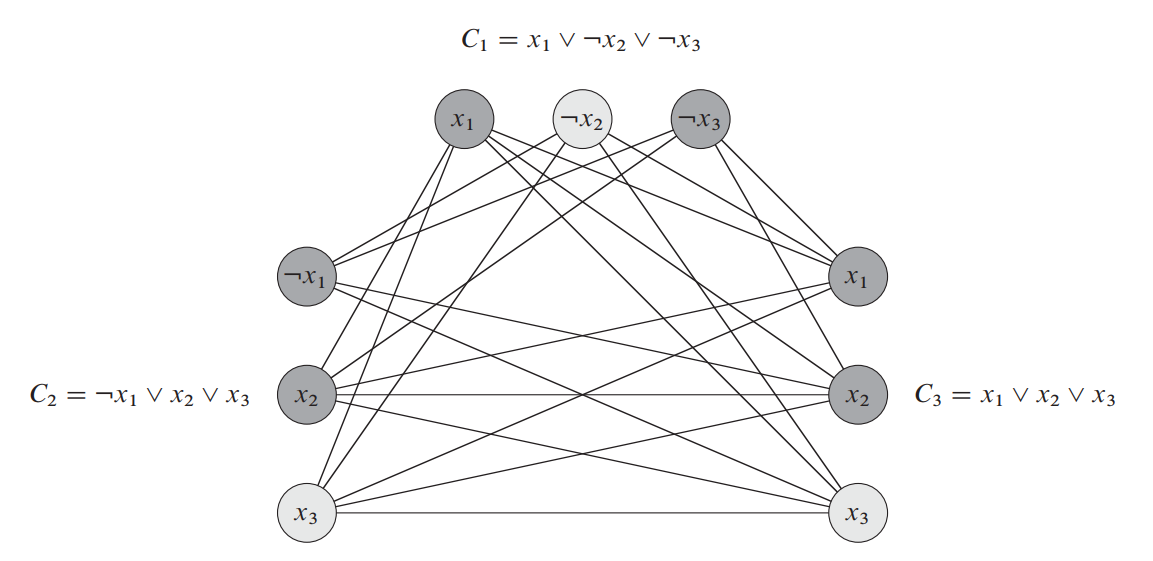
\includegraphics[scale=0.75]{imgs/clique.png}
\end{figure}

Podemos ver que los vértices con $\neg x_2$ y $x_3$, pintados de gris claro en la gráfica corresponden a los vértices que conforman en el clique.

\newpage
\subsection{Algoritmo}

\begin{itemize}
    \item Fase Adivinadora\\

    Por cada vértice $v\in V$ lanzamos una moneda, si cae sol agregamos $v$ a $V'$ que será el conjunto de vértices de la subgráfica que veremos que sea un clique y si cae águila no lo agregamos a $V'$.
    
    \item Fase Verificadora\\

    Si para cada vértice $v \in V'$ existe una arista $(u,v) \in E$ que conecta $v$ con todos los demás vértices $u \in V'$ decimos que el candidato a solución $V'$ creado en la fase adivinadora si es un clique y regresa SI, en otro caso regresa NO. 
    
\end{itemize}

\subsection{Técnica para la demostración del problema}

Reemplazo local.

\subsection{Aplicación en la vida real}
\begin{itemize}
    \item Optimización del compilador.
    \item Geometría computacional.
    \item Estadística aplicada.
\end{itemize}

\newpage
\section{Referencias}
\noindent
\begin{enumerate}
    \item Zhuoli Xiao. (2014). On Variants of Clique Problems and their Applications. 43-44.
\end{enumerate}

% \cite{DUMMY1} % example citation. remove for real assignment

% %------------------------------------------------

%\bibliographystyle{acm}
%\bibliography{references} % citation records are in the references.bib document

\end{document}
